\documentclass[UTF8,a4paper,11pt,fontset=fandol]{ctexart}
\usepackage[margin=2.35cm]{geometry}
\usepackage{amsmath,amssymb,booktabs,graphicx,array,tabularx}
\usepackage[numbers,sort&compress]{natbib}
\usepackage[hidelinks]{hyperref}
\usepackage{xurl}
\usepackage{caption,placeins}
\captionsetup{font=small,labelfont=bf}
\bibliographystyle{gbt7714-numerical}
\setlength{\parindent}{2em}
\setlength{\parskip}{0.25em}
\renewcommand{\arraystretch}{1.15}
\title{\bfseries 越复杂越好？\\[6pt]\large 基于 ETTh1 的油温单变量长序列预测研究}
\author{匿名作者}
\date{}

\begin{document}
\maketitle
\begin{abstract}
长序列预测中，网络结构与输入水平处理会共同影响误差。以 ETTh1 小时级油温为对象，采用固定的训练、验证与测试划分，比较局部均值、岭回归、多层感知机、循环网络、分解线性模型和片段 Transformer。实验区分绝对值预测与局部水平锚定，并分别报告三种子指标均值和预测集成结果。在历史与预测均为 96 h 的设置下，锚定岭回归的平均绝对误差为 1.632 ℃；锚定分解线性模型为 1.635 ℃，两种片段 Transformer 为 1.644 ℃ 与 1.655 ℃。局部水平处理减少了多种模型在低温测试段上的平均偏差。片段 Transformer 的三种子预测集成达到 1.600 ℃，说明集成效果需要单独评价。延长预测长度后，锚定岭回归在 192、336、720 h 的平均绝对误差分别为 1.914、2.129、2.116 ℃。负载输入、延长历史与注意力替换实验显示，输入信息、模型容量和参考水平需要分别控制。现有结果支持将局部水平锚定岭回归作为该固定划分下的低成本对照，并保留神经模型集成在部分指标上的优势。

\vspace{0.5em}
\noindent\textbf{关键词：}油温预测；长序列预测；ETTh1；岭回归；局部水平锚定；模型比较
\end{abstract}

\section*{Abstract}
Forecasting architecture and local-level handling jointly affect long-term prediction errors. We study hourly oil-temperature forecasting on ETTh1 using a fixed chronological split. Local means, Ridge regression, multilayer perceptrons, recurrent networks, DLinear, and patch-based Transformers are compared with explicit descriptions of preprocessing and model construction. Metrics averaged over three random seeds are reported separately from metrics of averaged predictions. For a 96-hour input and forecast horizon, anchored Ridge achieves a mean absolute error (MAE) of 1.632 degrees Celsius, compared with 1.635 for anchored DLinear and 1.644 and 1.655 for two anchored PatchTST configurations. Local-level handling reduces systematic bias on the colder test period. A three-seed PatchTST prediction ensemble reaches an MAE of 1.600, demonstrating the need to evaluate ensembling separately. Anchored Ridge obtains MAEs of 1.914, 2.129, and 2.116 at horizons of 192, 336, and 720 hours. Additional load channels, longer histories, and attention replacement are examined with their implementation-specific controls. The results support anchored Ridge as a low-cost reference for this split while retaining the advantages of neural prediction ensembles on selected metrics.

\section{引言}
电力变压器油温反映设备的热状态。预测未来数小时至数日的油温变化，有助于研究负载调度与温度预警。公开的电力变压器数据集（Electricity Transformer Dataset, ETT）包含油温和负荷记录，其中 ETTh1 为小时级子集\cite{informer2021,etdataset2021}。油温既有季节变化，也有短时波动；在历史油温预测未来油温的单变量任务中，模型需要同时确定未来温度的平均水平与随时间变化的形状。

长序列预测（Long-term Time-Series Forecasting, LTSF）已有多种建模方法。Informer 采用稀疏注意力\cite{informer2021}，Autoformer 引入序列分解\cite{autoformer2021}，FEDformer 在频域处理序列\cite{fedformer2022}。PatchTST 把连续观测组织为片段，再学习片段之间的关系\cite{patchtst2023}。这些设计改变了模型处理长历史的方式，也增加了需要控制的结构与训练因素。

线性与稠密网络提供了另一组对照。DLinear 用移动平均分解和两个线性映射完成多步预测\cite{dlinear2023}；TiDE 和 TSMixer 分别研究稠密编码与多层感知机混合\cite{tide2023,tsmixer2023}。可逆实例归一化（Reversible Instance Normalization, RevIN）则从输入窗口的均值与尺度入手处理分布变化\cite{revin2022}。因此，比较预测器时，需要同时说明输入表示、归一化、模型容量及模型选择方法。

ETTh1 的固定时间划分使这一问题尤其具体。训练段约覆盖一年，测试段覆盖 2017 年 10 月下旬至次年 2 月；训练与测试油温均值约为 17.13 ℃ 与 4.85 ℃。采用训练段全局统计量后，模型仍需适应低温测试段。最近一天的观测均值能够提供当前水平，因此将预测拆分为“局部水平加未来偏移量”，具有明确的数据依据。

本研究比较同一任务中的绝对值预测与局部水平锚定，分析结构差异与水平处理各自对应的误差变化。历史长度默认 96 h，预测长度取 96、192、336、720 h；额外实验考察六个负载通道、336 h 历史以及自注意力替换。主要结果来自已保存的逐种子指标、逐预测步误差和配对比较，神经模型的单次训练与三模型集成分别呈现。

研究围绕三个问题展开：第一，局部水平处理能减少多少系统偏差；第二，完成水平处理后，不同预测器还存在多大误差差异；第三，负载通道、长历史和片段交互机制的变化能否提供额外信息。对应实验同时保留参数量、种子波动与置信区间，支持读者评估比较的适用范围。

\section{相关工作}
\subsection{长序列预测方法}
长历史压缩与未来序列生成是长序列模型的两个基本环节。Transformer 方法通过稀疏注意力、序列分解或频域处理降低长序列计算开销\cite{informer2021,autoformer2021,fedformer2022}。PatchTST 将相邻时刻组成片段，以片段作为注意力输入；其通道独立设计对每个变量分别编码\cite{patchtst2023}。本研究使用单变量片段编码器，并明确列出局部实现的片段数、嵌入宽度及预测头。

分解线性模型与循环网络分别提供线性映射和状态递推对照。DLinear 将移动平均趋势与剩余项分别映射到预测区间\cite{dlinear2023}。SegRNN 使用片段级循环和并行多步预测，减少逐时刻递推次数\cite{segrnn2023}。本文对这两类模型分别展开分解算子与并行解码过程，以比较它们处理历史信息的方式。

\subsection{水平处理与评价}
窗口间的均值与尺度变化会改变模型接收的输入分布。RevIN 使用输入窗口均值与标准差进行归一化，并在输出端恢复尺度\cite{revin2022}。本研究的局部水平锚定仅减去最近 24 h 的均值，保留残差幅度；另以窗口均值与标准差归一化作补充对照。两者使用的时间范围与尺度处理不同，结果分别报告。

预测评价还受到时间划分、滚动窗口及重复观测的影响\cite{hewamalage2022}。本研究采用固定行索引划分，目标完整落在所属数据段内，输入可以使用前一段的已观测历史。相邻窗口共享大量观测，因此配对误差采用连续块重采样；不同随机种子的波动单独统计。这些处理用于描述两类不同的不确定性。

\section{数据与实验协议}
\subsection{数据与质量问题}
原始文件包含 17,420 行，时间范围为 2016-07-01 00:00 至 2018-06-26 19:00，时间间隔为 1 h。字段包含六个负荷变量和油温 OT；时间戳无重复，数值无 NaN。图~\ref{fig:split} 展示完整序列与实验使用的时间段，低温测试段与训练段的水平差异直接可见。

\begin{figure}[tbp]
\centering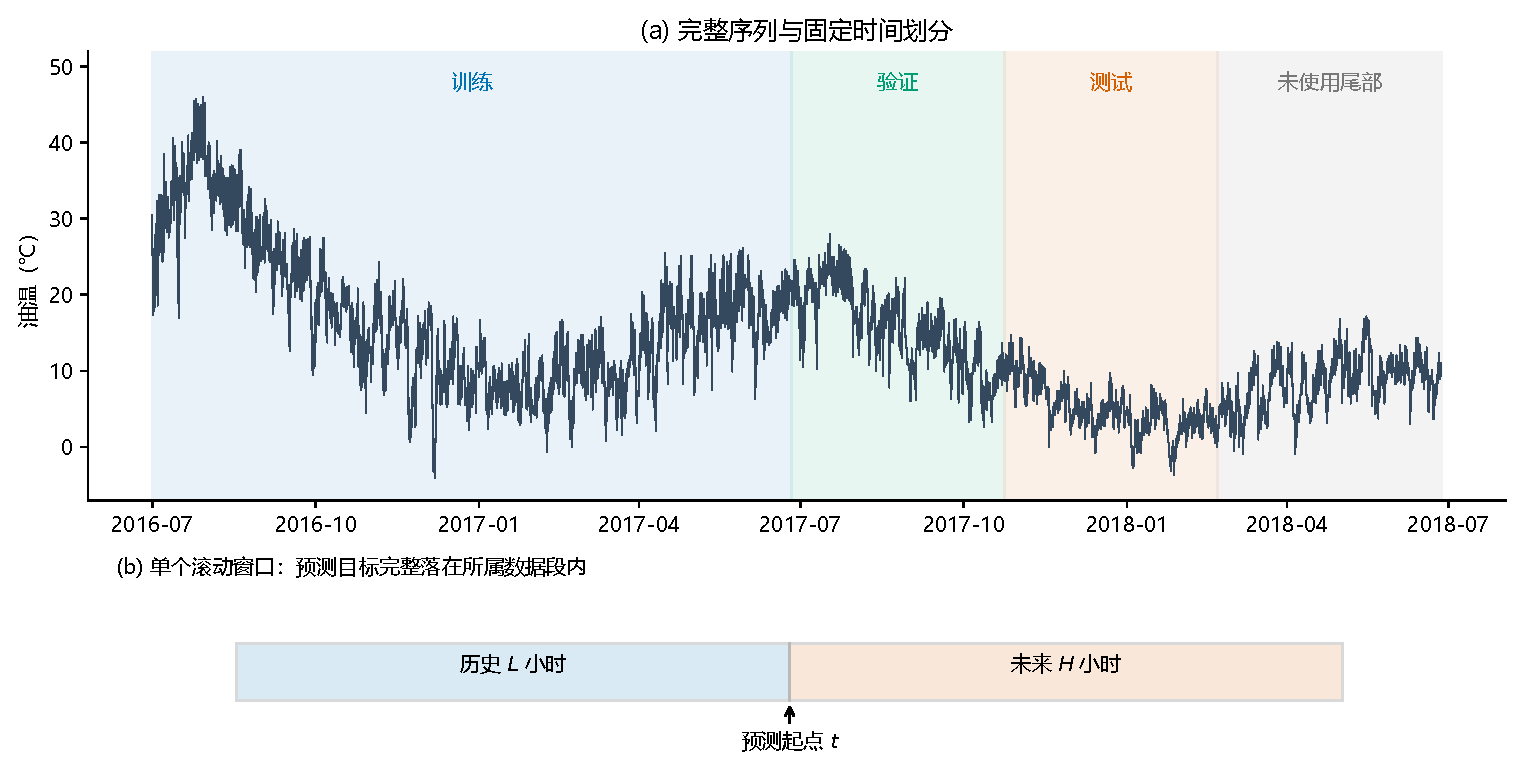
\includegraphics[width=\linewidth]{figures/fig0_split.pdf}
\caption{油温序列、时间划分与滚动窗口。上图阴影表示训练、验证、测试及未使用尾部；下图表示一个预测起点对应的历史与目标。验证和测试输入可跨越前一段边界，预测目标保持在所属数据段内。}
\label{fig:split}
\end{figure}

质量检查发现，所有含 31 日的月份都出现整日七列冻结，共 14 天、336 行。标准测试段中含 3 个冻结日，即 72 行，占该段 2.5\%。此外，训练段在 2016 年 12 月存在负荷零值块，验证段的两个低负荷通道存在 141 h 恒值块。这些常量与零值按采集伪影记录；当前实验保留原始数值，因此结果反映含伪影数据上的预测误差。

\subsection{任务与滚动窗口}
设小时油温为 $y_t$，历史长度为 $L$，预测长度为 $H$，单变量输入与目标定义为
\begin{equation}
\mathbf{x}_t=(y_{t-L+1},\ldots,y_t)^\top\in\mathbb R^L,\qquad
\mathbf{y}_t=(y_{t+1},\ldots,y_{t+H})^\top\in\mathbb R^H.
\label{eq:task}
\end{equation}
单变量设置记为 S 模式。默认 $L=H=96$，即根据过去 4 天预测未来 4 天。模型一次生成全部 $H$ 个输出；预测期间使用同一输入窗口，逐步误差可按未来小时位置分别统计。

固定划分以每月 30 天换算，行索引与日期见表~\ref{tab:split}。末尾 3,020 行不参与；测试时间覆盖晚秋至冬季。每次预测起点前移 1 h，仅保留目标完整落在对应段内的窗口，因此训练窗口数为 $8640-L-H+1$，验证与测试各为 $2880-H+1$。

\begin{table}[tbp]
\centering\small
\caption{固定划分与默认 96 h 历史、96 h 预测的样本数。日期均含末日 23:00。训练段前 96 h 仅用于构造首个输入。}
\label{tab:split}
\begin{tabular}{lrrll}
\toprule 数据段 & 行数 & 窗口数 & 行索引 & 日期范围\\\midrule
训练 & 8,640 & 8,449 & $[0,8640)$ & 2016-07-01 至 2017-06-25\\
验证 & 2,880 & 2,785 & $[8640,11520)$ & 2017-06-26 至 2017-10-23\\
测试 & 2,880 & 2,785 & $[11520,14400)$ & 2017-10-24 至 2018-02-20\\\bottomrule
\end{tabular}
\end{table}

额外负载实验采用多变量输入、单变量输出的 MS 模式。输入为 $L\times7$ 矩阵，预测目标仍为未来油温。长历史实验取 $L=336$、$H=96$；验证与测试目标及预测起点保持相同，训练窗口数降至 8,209。该设置为输入信息与历史长度比较提供共同的目标集合。

\subsection{标准化与模型选择}
所有固定尺度统计量均在训练窗口上拟合。按滞后标准化为输入的每个小时位置分别估计均值与标准差；按变量标准化则将所有训练窗口的时间位置合并，每个变量使用一个均值与标准差。表~\ref{tab:scale} 给出各实现采用的方式。

\begin{table}[tbp]
\centering\small
\caption{实际实现的标准化方式。目标标准化发生在锚定之后；预测时先反标准化，再恢复输入窗口的参考水平。}
\label{tab:scale}
\begin{tabularx}{\linewidth}{lXX}
\toprule 模型 & 输入尺度 & 目标尺度\\\midrule
96 h 岭回归 & 按滞后 & 保留油温残差单位\\
MLP、PatchTST、片段混合 MLP & 按滞后 & 按预测步\\
GRU、LSTM & 单变量合并时间位置 & 按预测步\\
DLinear、SegRNN & 单变量合并时间位置 & 合并全部预测步\\
192/336/720 h 岭回归 & 按滞后 & 按预测步\\
MS 岭回归及其 S 对照 & 按变量 & 合并全部预测步\\\bottomrule
\end{tabularx}
\end{table}

岭回归正则化强度取 $\{0.1,1,10,100,1000\}$，按验证集平均绝对误差（Mean Absolute Error, MAE）选择。神经模型使用均方误差（Mean Squared Error, MSE）损失和 Adam 优化器。学习率为 $10^{-3}$，权重衰减为 $10^{-4}$，批量大小为 256，梯度范数裁剪阈值为 1。最多训练 300 轮，验证 MAE 连续 20 轮未改善时停止，并恢复验证 MAE 最低的参数。随机种子取 0、1、2，训练设备为 RTX 5090 Laptop GPU，软件为 PyTorch 2.14.1 与 CUDA 13.0。

预处理尽量沿用各轮已完成的实现，因此表~\ref{tab:scale} 中仍存在尺度处理差别。水平处理的对照在同一模型内部进行；负载输入实验另外设置同尺度 S 对照。跨家族结果用于比较这些具体训练方案的总体误差，结构作用的讨论结合对应消融进行。

\subsection{指标与统计比较}
设测试窗口数为 $N$，误差 $e_{i,h}=\hat y_{i,h}-y_{i,h}$，则
\begin{equation}
\mathrm{MSE}=\frac{1}{NH}\sum_{i,h}e_{i,h}^2,\quad
\mathrm{MAE}=\frac{1}{NH}\sum_{i,h}|e_{i,h}|,\quad
\mathrm{Bias}=\frac{1}{NH}\sum_{i,h}e_{i,h}.
\end{equation}
MSE 单位为 ℃$^2$，MAE 与平均偏差单位为 ℃。所有主结果在恢复原始油温单位后计算；正偏差表示整体高估。相对基线的 MAE 改善率定义为 $1-\mathrm{MAE}_{\rm model}/\mathrm{MAE}_{\rm ref}$，正值表示误差较低。

三种子指标均值是先计算每次训练的指标，再对三个数取平均；其标准差使用样本标准差。预测集成则先计算 $\hat{\mathbf y}^{\rm ens}=\frac13\sum_{s=1}^3\hat{\mathbf y}^{(s)}$，再计算指标。误差中的绝对值与平方使两者通常不同，因此分别报告。

配对比较先在每个窗口上计算两个模型的 MAE 或 MSE 差，再沿预测起点序列抽取连续 96 个窗口组成的块。每次有放回抽块，拼接并截取至原样本数，重复 2,000 次，取均值差的 2.5\% 和 97.5\% 分位数作为区间。本文沿用已保存的块长；当 $H>96$ 时，目标重叠可能延续到更远起点，区间解释需结合这一依赖长度。

步内去偏误差以 $\bar e_h=N^{-1}\sum_i e_{i,h}$ 为每个预测步的平均误差，计算 $e_{i,h}-\bar e_h$ 的 MSE 或 MAE。由于 $\bar e_h$ 使用测试真值，该指标仅用于诊断水平误差，在预测阶段不参与校正。主结果仍使用未经测试标签校正的预测。

\FloatBarrier
\section{预测模型构建}
\subsection{局部水平与统计基线}
统计基线直接沿用当前油温水平或最近的变化模式。最后值预测将 $y_t$ 重复 $H$ 次；$q$ 小时局部均值预测定义为
\begin{equation}
\ell_t^{(q)}=\frac1q\sum_{j=0}^{q-1}y_{t-j},\qquad
\hat{\mathbf y}_t=\ell_t^{(q)}\mathbf1_H,\quad q\in\{24,96\}.
\end{equation}
日周期复制则按顺序循环使用最近 24 h 的观测。这些名称直接描述预测规则，后续比较统一采用“最后值”“24 h 均值”“96 h 均值”和“日周期复制”。

局部水平锚定取 $\ell_t=\ell_t^{(24)}$，构造
\begin{equation}
\mathbf x_t^c=\mathbf x_t-\ell_t\mathbf1_L,\qquad
\mathbf y_t^c=\mathbf y_t-\ell_t\mathbf1_H.
\label{eq:center}
\end{equation}
训练时参考水平由输入计算，目标与输入减去同一数值；预测时模型生成未来相对该水平的偏移量，再加回 $\ell_t$。图~\ref{fig:pipeline} 将参考水平作为独立支路接入输出端，说明中心化输入和恢复水平使用同一历史统计量。

\begin{figure}[tbp]
\centering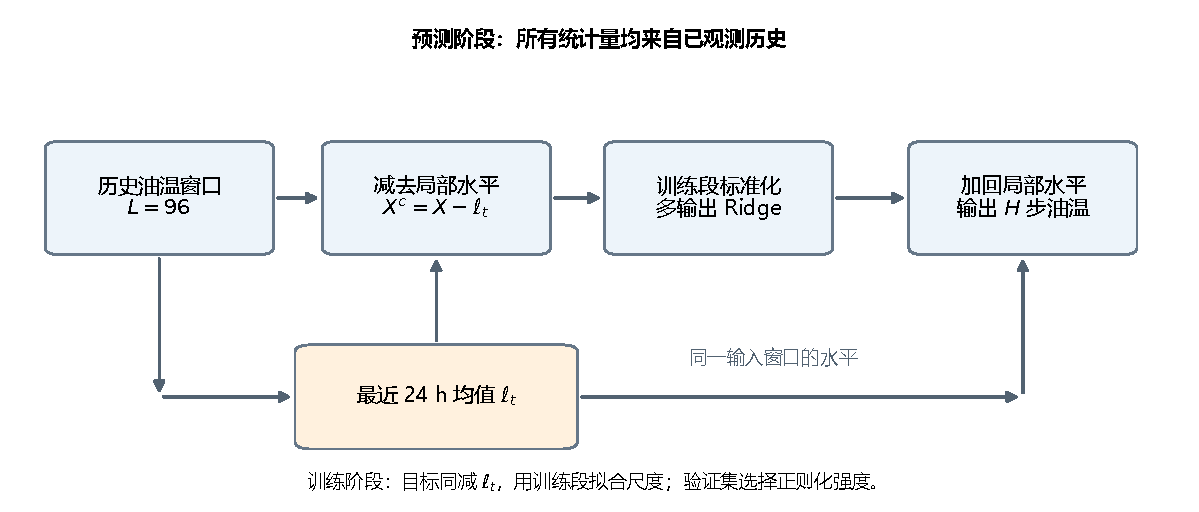
\includegraphics[width=\linewidth]{figures/fig1_pipeline.pdf}
\caption{局部水平锚定岭回归的预测流程。历史输入分成残差建模与水平恢复两条支路。图中预测头输出油温残差；96 h 主实验的目标保留原单位，长预测实验则在头部输出后先完成目标反标准化。}
\label{fig:pipeline}
\end{figure}

\subsection{多输出岭回归}
多输出岭回归用同一历史窗口分别拟合各个未来小时的温度。对 $n$ 个训练窗口，按滞后标准化后的输入矩阵记为 $Z\in\mathbb R^{n\times L}$，目标残差记为 $R\in\mathbb R^{n\times H}$。参数 $W\in\mathbb R^{L\times H}$ 与 $b\in\mathbb R^H$ 通过
\begin{equation}
\min_{W,b}\ \|R-ZW-\mathbf1_n b^\top\|_F^2+\alpha\|W\|_F^2
\label{eq:ridge}
\end{equation}
求解。截距不受惩罚；每个预测步有一组历史权重。预测为 $\hat{\mathbf y}_t=W^\top\mathbf z_t+b+\ell_t\mathbf1_H$，因此 96 h 历史到 96 h 输出含 $96\times96+96=9,312$ 个回归系数与截距。

若输入整体加上常数 $c$，局部均值也增加 $c$，中心化输入保持相同；固定标准化后的残差预测相同，最终输出增加 $c$。因此，该构造对输入整体平移具有等变性。它显式保留当前水平，使线性映射主要拟合未来偏移量。

当残差预测在原单位下为零时，模型退化为 24 h 均值预测。这给出一个易解释的参考点；实际拟合的权重由训练损失与正则化决定。带目标标准化时，零标准化输出对应训练目标残差均值，恢复原单位后需同时计入该均值。

\subsection{感知机与循环网络}
MLP 对整个窗口进行非线性映射，循环网络则按时间顺序更新状态。多层感知机（Multilayer Perceptron, MLP）采用两层 128 单元隐藏层：
\begin{equation}
h_1=\operatorname{ReLU}(A_1z+a_1),\quad
h_2=\operatorname{ReLU}(A_2h_1+a_2),\quad
\hat r=A_3h_2+a_3.
\end{equation}
默认尺寸依次为 $96\to128\to128\to96$，共 41,312 个参数。模型将整个窗口作为向量输入，直接学习历史位置之间的非线性组合。

门控循环单元（Gated Recurrent Unit, GRU）与长短期记忆网络（Long Short-Term Memory, LSTM）按小时顺序接收标量输入，均为单层、隐藏宽度 64。GRU 利用重置门和更新门控制历史状态，例如
\begin{equation}
r_j=\sigma(A_rx_j+U_rh_{j-1}+b_r),\quad
z_j=\sigma(A_zx_j+U_zh_{j-1}+b_z),\quad
h_j=(1-z_j)\odot\tilde h_j+z_j\odot h_{j-1},
\end{equation}
其中 $\sigma$ 为 sigmoid 函数，$\odot$ 表示逐元素乘积。候选状态为
\begin{equation}
\tilde h_j=\tanh\!\left(A_nx_j+a_n+r_j\odot(U_nh_{j-1}+b_n)\right).
\end{equation}
更新门控制候选状态与前一时刻状态的比例，因此 GRU 可在逐小时编码中保留较慢变化的信息。

LSTM 另外维护记忆单元 $c_j$。令输入门、遗忘门、输出门分别为 $i_j,f_j,o_j$，各门均对当前输入与上一隐藏状态的仿射变换使用 sigmoid。候选记忆 $g_j$ 则使用双曲正切函数，状态更新为
\begin{equation}
c_j=f_j\odot c_{j-1}+i_j\odot g_j,\qquad
h_j=o_j\odot\tanh(c_j).
\end{equation}
两种循环网络均从零初始状态编码历史，取最后隐藏状态 $h_L\in\mathbb R^{64}$，接 $64\to H$ 线性头。GRU 与 LSTM 分别含 19,104 和 23,392 个参数，作为两种门控状态设计的对照。

循环计算发生在历史编码阶段，输出端一次生成 $H$ 个值。绝对值版本在全局标准化空间预测油温，锚定版本在式~\eqref{eq:center} 的残差空间预测，再恢复水平。这样可在相同循环结构内部检查水平处理对误差的作用。

\subsection{分解线性模型}
DLinear 对平滑趋势与短时残差分别预测，再合并两个分支。先对标准化输入做宽度 25、步长 1 的移动平均，在两端各重复边界值 12 次以保持长度。令该线性平滑算子为 $M$，则趋势 $T=Mz$，剩余项 $S=z-T$，预测为
\begin{equation}
\hat r=A_TT+a_T+A_SS+a_S.
\label{eq:dlinear}
\end{equation}
两个线性头均为 $96\to96$，总参数量为 18,624；两支输出逐步相加后恢复原单位和参考水平。

移动平均与两个预测头均为线性或仿射映射，因此式~\eqref{eq:dlinear} 可写成 $[A_TM+A_S(I-M)]z+a_T+a_S$。这说明本实现仍属于仿射预测器，其差异主要来自参数化、分支优化与正则化。该性质为它与岭回归接近的结果提供结构解释。

\subsection{片段 Transformer}
PatchTST 将相邻小时组织为连续片段，以片段作为注意力输入\cite{patchtst2023}。将标准化序列按长度 $P=16$、步长 $S=8$ 切成重叠片段，片段数为
\begin{equation}
N_p=\left\lfloor\frac{L-P}{S}\right\rfloor+1.
\end{equation}
$L=96$ 时得到 11 个片段，$L=336$ 时得到 41 个片段。实现使用完整片段，无尾部补片段；每个片段经 $16\to d$ 线性嵌入并加可学习位置向量。输入张量从 $B\times L$ 变为 $B\times N_p\times d$，其中 $B$ 为批量大小。

每个编码块使用前置层归一化。令输入为 $U$，则
\begin{align}
V&=U+\operatorname{Dropout}(\operatorname{MHA}(\operatorname{LN}(U))),\\
U^+&=V+\operatorname{Dropout}(\operatorname{FFN}(\operatorname{LN}(V))).
\end{align}
多头自注意力（Multi-Head Attention, MHA）使用 4 个头；单头以 $\operatorname{softmax}(QK^\top/\sqrt{d_k})V_h$ 聚合片段表示。前馈网络（Feed-Forward Network, FFN）为 $d\to d_{\rm ff}\to d$，使用 GELU 激活。编码后展平所有片段，接 dropout 和 $N_pd\to H$ 线性头，完成直接多步预测。

\begin{figure}[tbp]
\centering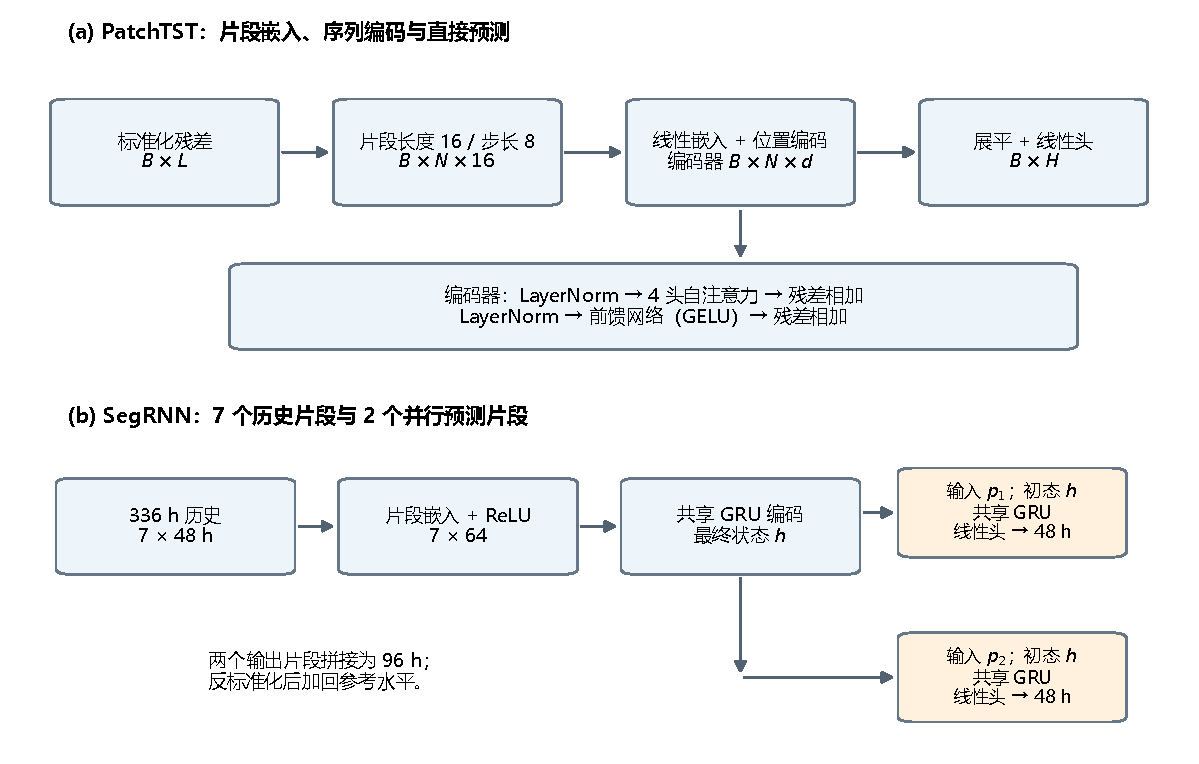
\includegraphics[width=\linewidth]{figures/fig5_architectures.pdf}
\caption{两类片段模型的局部实现。PatchTST 沿片段序列编码，张量尺寸随历史长度变化；SegRNN 将 7 个历史片段压缩为状态，再以两个位置向量并行生成未来片段。两种结构均在输出端恢复输入窗口的参考水平。}
\label{fig:architecture}
\end{figure}

图~\ref{fig:architecture}(a) 给出片段编码到预测头的连接，表~\ref{tab:patch} 区分已运行的配置。64 维、2 层模型用于绝对值、24 h 锚定与窗口均值尺度归一化比较；16 维、3 层模型用于注意力消融和长历史比较。两组配置在本文始终按嵌入宽度标记，分别对应独立的模型与结果。

\begin{table}[tbp]
\centering\small
\caption{PatchTST 实际配置。各配置均为 4 头注意力，编码与预测头 dropout 均为 0.1。参数量包含嵌入、位置向量、编码块和输出头。}
\label{tab:patch}
\begin{tabular}{rrrrrrl}
\toprule $L$ & $H$ & $d$ & 层数 & $d_{\rm ff}$ & 参数量 & 用途\\\midrule
96 & 96 & 64 & 2 & 128 & 136,416 & 水平处理比较\\
96 & 96 & 16 & 3 & 32 & 24,112 & 片段交互对照\\
336 & 96 & 16 & 3 & 32 & 70,672 & 历史长度比较\\\bottomrule
\end{tabular}
\end{table}

\subsection{片段交互替换}
片段交互对照比较内容相关的注意力权重与固定参数映射。保留 16 维 PatchTST 的嵌入、位置编码、三层深度、前馈网络和预测头，将自注意力替换为跨片段 MLP。对 $B\times11\times16$ 的归一化表示，先转置为 $B\times16\times11$，沿片段轴应用 $11\to48\to11$ 的 GELU 网络，再转置回原形状并残差相加。

该模型各特征共享片段混合映射，dropout 为 0.1，其余训练设置沿用注意力版本。替换后的总参数量为 24,193，比注意力版本多 81，约为 0.34\%。因此，这组实验在近似相同容量下比较内容相关注意力与固定参数片段映射，结果用于判断该小配置的片段交互需求。

\subsection{片段循环网络}
SegRNN 在片段之间更新循环状态，并行生成多个未来片段\cite{segrnn2023}。输入为 336 h，按 48 h 划为 7 个非重叠片段。每段经 $48\to64$ 线性层和 ReLU 转为 64 维表示，单层 GRU 依次处理 7 段，得到最终状态 $h\in\mathbb R^{64}$。

未来 96 h 分成两个 48 h 片段。解码时把同一状态 $h$ 复制给两个分支，每个分支使用独立的可学习位置向量 $p_j\in\mathbb R^{64}$ 作为单步 GRU 输入；编码与解码共享 GRU 参数。两个解码状态分别经过 dropout 与 $64\to48$ 的线性头，再拼接为 96 维输出。图~\ref{fig:architecture}(b) 展示这两个并行分支，共含 31,344 个参数。

该实现比较两种参考水平：最近 24 h 均值，以及最后观测值。后者按 $x-y_t$ 和 $Y-y_t$ 构造残差，接近 SegRNN 的末值参考思路；两者均以训练窗口拟合固定尺度。它们用相同结构检验参考水平与分段循环预测之间的关系。

\FloatBarrier
\section{实验结果与分析}
\subsection{水平处理与预测误差}
主实验固定输入与输出长度，先比较局部水平处理，再比较模型结构。默认 96 h 输入、96 h 输出下，最后值、24 h 均值、96 h 均值的测试 MAE 分别为 1.865、1.820、1.821 ℃。24 h 均值在这组基线中略低；后续长预测另外保留 96 h 均值作对照。表~\ref{tab:main} 由保存的测试指标自动生成，以同一位数呈现各模型结果。

\begin{table}[tbp]
\centering\small\setlength{\tabcolsep}{4pt}
\caption{S 模式 96 h 输入、96 h 输出结果。神经模型报告三种子指标均值 $\pm$ 样本标准差；偏差为三种子均值。MSE 单位为 ℃$^2$，MAE 和偏差单位为 ℃。16 维 PatchTST 与片段混合 MLP 只运行了锚定版本。}
\label{tab:main}
\begin{tabular}{lccc}
\toprule 模型 & MSE & MAE & 平均偏差\\\midrule
Ridge（直接预测） & 5.107 & 1.670 & $+0.780$ \\
\textbf{Ridge（局部水平锚定）} & 4.613 & 1.632 & $+0.105$ \\
MLP（直接预测） & $12.198 \pm 1.314$ & $2.853 \pm 0.186$ & $+2.678$ \\
MLP（局部水平锚定） & $4.680 \pm 0.040$ & $1.663 \pm 0.006$ & $-0.034$ \\
GRU（直接预测） & $17.878 \pm 1.040$ & $3.532 \pm 0.120$ & $+3.331$ \\
GRU（局部水平锚定） & $4.776 \pm 0.208$ & $1.671 \pm 0.024$ & $-0.030$ \\
LSTM（直接预测） & $18.243 \pm 0.031$ & $3.565 \pm 0.003$ & $+3.339$ \\
LSTM（局部水平锚定） & $5.077 \pm 0.252$ & $1.759 \pm 0.044$ & $-0.202$ \\
DLinear（直接预测） & $6.224 \pm 0.245$ & $1.843 \pm 0.036$ & $+1.264$ \\
DLinear（局部水平锚定） & $4.616 \pm 0.004$ & $1.635 \pm 0.003$ & $+0.093$ \\
PatchTST 64维（直接预测） & $11.250 \pm 1.699$ & $2.712 \pm 0.262$ & $+2.330$ \\
PatchTST 64维（局部水平锚定） & $4.777 \pm 0.123$ & $1.655 \pm 0.035$ & $+0.084$ \\
PatchTST 16维（局部水平锚定） & $4.842 \pm 0.286$ & $1.644 \pm 0.034$ & $+0.301$ \\
片段混合 MLP（局部水平锚定） & $4.709 \pm 0.028$ & $1.684 \pm 0.005$ & $-0.010$ \\
\bottomrule

\end{tabular}
\end{table}

绝对值 MLP、GRU、LSTM 的 MAE 为 2.853、3.532、3.565 ℃，均高于局部均值。锚定后，它们分别降至 1.663、1.671、1.759 ℃；对应平均偏差从 2.678、3.331、3.339 ℃ 降至接近零或较小负值。图~\ref{fig:main}(b) 对相同结构进行配对展示，支持在本数据划分下优先处理水平差异。

\begin{figure}[tbp]
\centering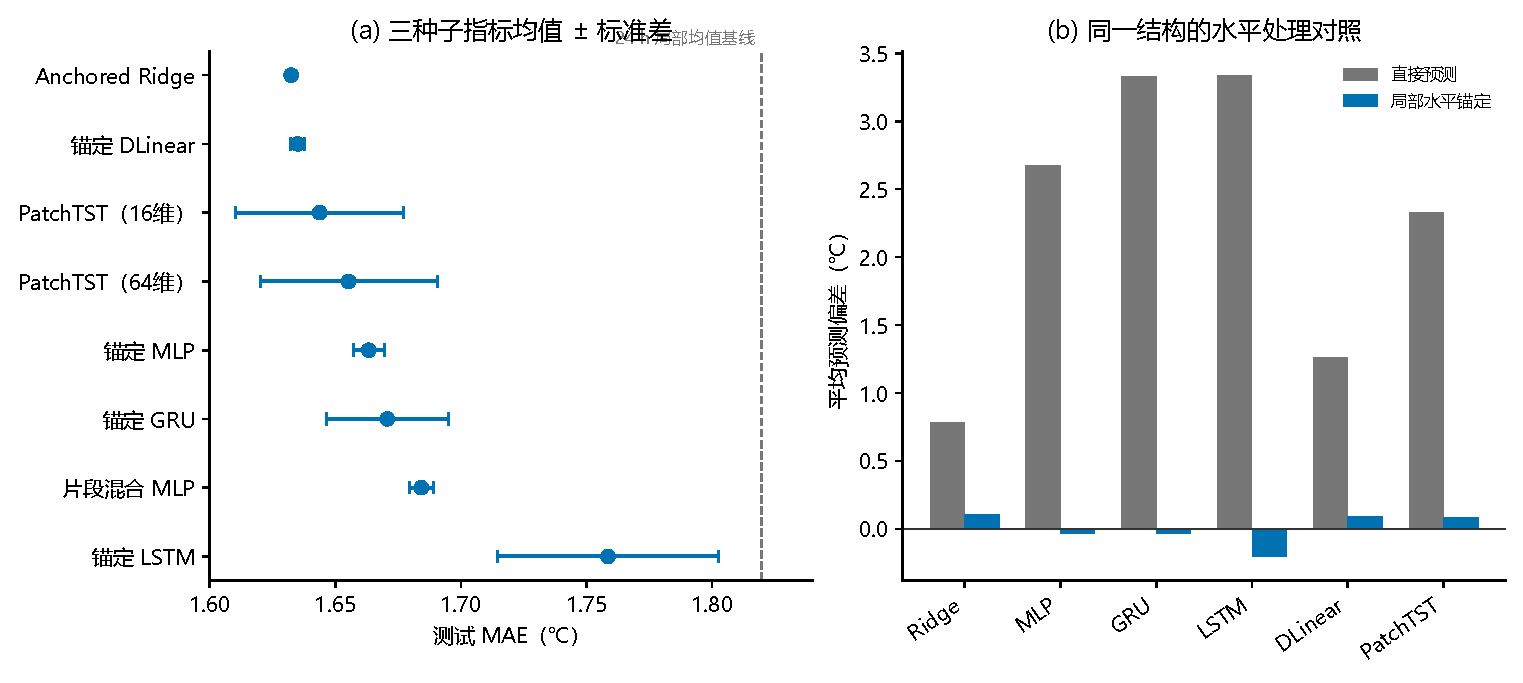
\includegraphics[width=\linewidth]{figures/fig2_main.pdf}
\caption{96 h 预测的误差与偏差。(a) 点表示三种子 MAE 均值，误差线表示种子标准差，岭回归为确定性结果；虚线为 24 h 均值基线。(b) 水平处理对照中的 PatchTST 采用 64 维、2 层配置。两图均使用 96 h 历史。}
\label{fig:main}
\end{figure}

锚定岭回归的 MSE 为 4.613、MAE 为 1.632 ℃，较绝对值岭回归分别降低约 9.7\% 和 2.2\%。锚定 DLinear 的 MAE 为 1.635 ℃，相差约 0.003 ℃。两种锚定 PatchTST 的三种子 MAE 均值为 1.644 与 1.655 ℃。这些差异小于多种神经模型自身的种子波动，因此保留简单线性预测器作为主要参考。

\subsection{预测集成与归一化}
输出平均可以抵消部分独立训练的预测波动。表~\ref{tab:ensemble} 将种子指标均值与预测集成并列。16 维 PatchTST 集成 MAE 为 1.600 ℃，低于锚定岭回归的点估计；锚定 GRU 集成的 MSE 为 4.525，也低于该岭回归。模型比较因此同时考虑所用模型数量与评价指标。

\begin{table}[tbp]
\centering\small
\caption{三种子指标均值与预测集成。所有模型采用 96 h 历史和 24 h 均值锚定。指标均值表示三次独立训练的平均；集成表示三个预测向量平均后的结果。}
\label{tab:ensemble}
\begin{tabular}{lrrrr}
\toprule & \multicolumn{2}{c}{种子指标均值} & \multicolumn{2}{c}{预测集成}\\
模型 & MSE & MAE & MSE & MAE\\\midrule
MLP & 4.680 & 1.663 & 4.641 & 1.655\\
GRU & 4.776 & 1.671 & 4.525 & 1.624\\
LSTM & 5.077 & 1.759 & 4.864 & 1.722\\
DLinear & 4.616 & 1.635 & 4.607 & 1.633\\
PatchTST 64维 & 4.777 & 1.655 & 4.617 & 1.623\\
PatchTST 16维 & 4.842 & 1.644 & 4.632 & 1.600\\
片段混合 MLP & 4.709 & 1.684 & 4.585 & 1.660\\\bottomrule
\end{tabular}
\end{table}

64 维 PatchTST 还运行了窗口均值与标准差归一化：对每个窗口计算 $\mu_t$ 和 $s_t=\operatorname{std}(\mathbf x_t)+10^{-8}$，输入与目标均按这两个统计量变换，输出再乘 $s_t$ 并加 $\mu_t$。该版本三种子 MAE 为 1.669 ℃，24 h 均值锚定为 1.655 ℃。这项具体实现采用固定的窗口统计恢复，结果支持把均值处理与尺度处理分别检验。

\subsection{延长预测长度}
长预测实验保持历史长度相同，分别拟合不同长度的未来残差。保持 $L=96$，每个 $H$ 独立拟合岭回归并以验证 MAE 选择正则化强度。表~\ref{tab:horizon} 给出各自全部有效测试窗口，四个预测长度均选中 $\alpha=100$。192 h 额外运行的锚定 PatchTST 三种子 MAE 为 1.993 ℃，集成为 1.935 ℃，该长度的岭回归为 1.914 ℃。

\begin{table}[tbp]
\centering\small
\caption{96 h 历史下的跨预测长度结果。每行使用对应长度的全部有效测试窗口。MAE 改善率以同一行的 96 h 均值为参考。336 h 与 720 h 的模型比较仅包含岭回归和统计基线。}
\label{tab:horizon}
\begin{tabular}{rrrrrr}
\toprule $H$ & 窗口数 & Ridge MSE & Ridge MAE & 均值 MAE & MAE 改善率\\\midrule
96 & 2785 & 4.613 & 1.632 & 1.821 & 10.37\% \\
192 & 2689 & 6.178 & 1.914 & 2.063 & 7.23\% \\
336 & 2545 & 7.310 & 2.129 & 2.275 & 6.43\% \\
720 & 2161 & 7.092 & 2.116 & 2.395 & 11.65\% \\
\bottomrule

\end{tabular}
\end{table}

预测长度增大时，有效起点数从 2,785 降至 2,161，因此表中跨行差异同时包含目标长度和起点集合变化。图~\ref{fig:horizon}(a) 改用 720 h 实验保存的 2,161 个共同起点结果：岭回归 MAE 随 $H$ 从 96 增至 720，依次为 1.594、1.892、2.072、2.116 ℃。在共同起点下，336 h 至 720 h 的平均误差仍增加，但增幅较前两个区间小。

\begin{figure}[tbp]
\centering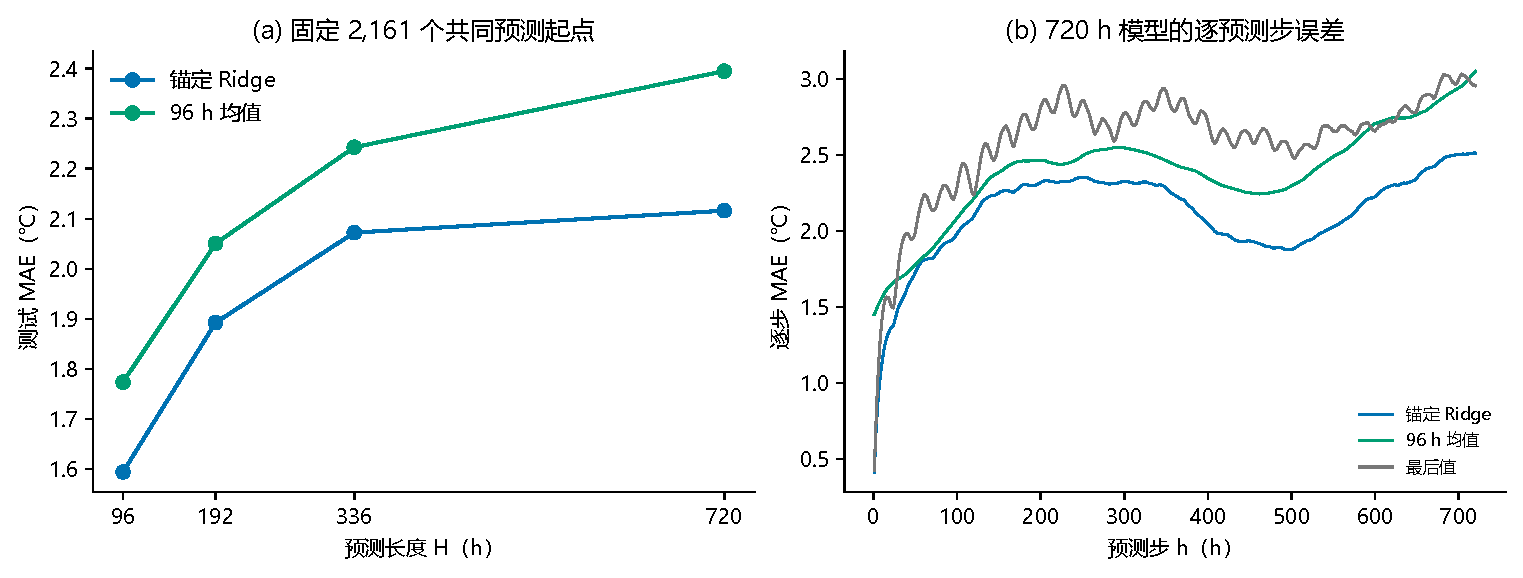
\includegraphics[width=\linewidth]{figures/fig3_horizon.pdf}
\caption{长预测的两个观察角度。(a) 每个预测长度独立拟合模型，在相同 2,161 个预测起点上计算整个目标区间的平均 MAE。(b) 固定 720 h 模型，分别计算第 $h$ 小时误差。前者考察整个区间，后者展示未来位置变化，两者分别解释。}
\label{fig:horizon}
\end{figure}

720 h 模型的平均偏差仍为 +0.604 ℃，说明当前水平恢复后，远期温度变化仍有系统性误差。逐步误差曲线也保留较大的远期波动。因此，现有实验支持锚定岭回归在长预测中优于所比较的局部水平基线，并提示继续研究随季节变化的未来水平。

\subsection{负载输入与历史长度}
输入消融分别增加负载通道与历史小时数。七通道岭回归只对 OT 减去局部油温均值，其他负载通道保留原值，再按变量标准化并展平为 672 维输入。对应的单变量对照同样采用按变量标准化，MAE 为 1.633 ℃；七通道版本为 1.795 ℃。配对 MAE 差为 +0.163 ℃，95\% 区间为 $[+0.113,+0.226]$ ℃，因此当前线性输入拼接方案保留单变量设置。

\begin{figure}[tbp]
\centering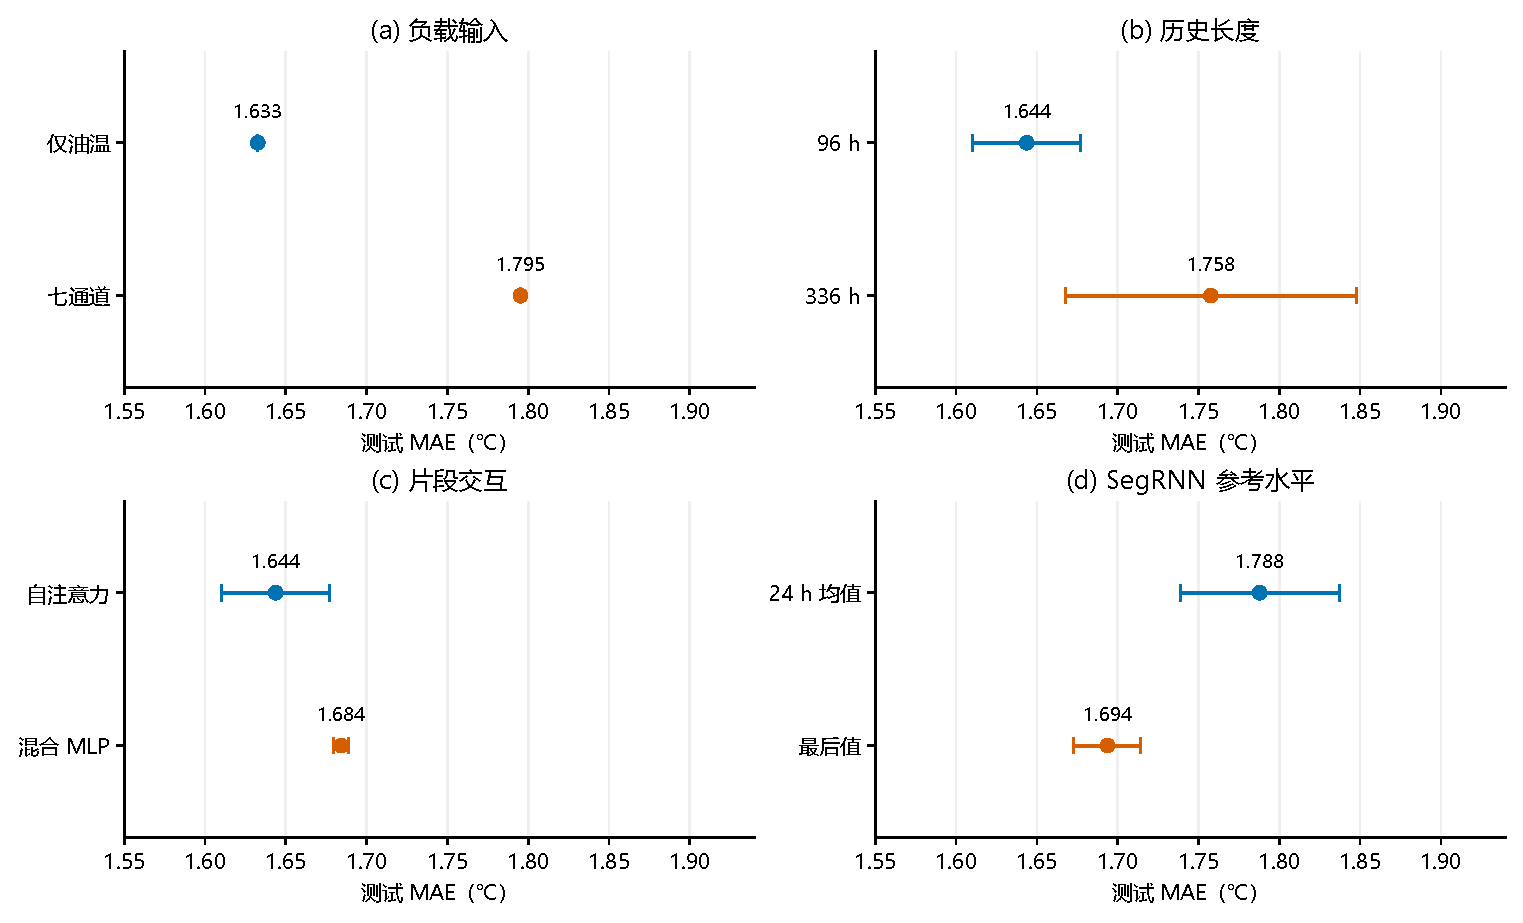
\includegraphics[width=\linewidth]{figures/fig4_ablations.pdf}
\caption{四组消融的测试 MAE。神经模型点为三种子指标均值，误差线为种子标准差；确定性岭回归无种子误差线。历史长度图采用 16 维 PatchTST，SegRNN 图采用 336 h 历史。种子误差线与正文的窗口块重采样区间描述不同的波动来源。}
\label{fig:ablation}
\end{figure}

历史长度比较如图~\ref{fig:ablation}(b)。岭回归从 96 h 延长至 336 h 后，MAE 由 1.632 降至 1.625 ℃，配对差区间为 $[-0.152,+0.112]$ ℃，逐窗口胜率约 49.6\%。16 维 PatchTST 的三种子 MAE 从 1.644 升至 1.758 ℃；预测集成从 1.600 升至 1.692 ℃，配对集成 MAE 差区间为 $[-0.070,+0.230]$ ℃。因此，已测长历史方案未提供明确的误差降低证据。

延长历史也将 PatchTST 片段数从 11 增为 41，参数量从 24,112 增至 70,672。三个长历史种子均在第 1 轮取得最低验证 MAE，随后在耐心轮数内停止训练。该结果同时涉及更长输入、更宽展平预测头和较少训练窗口，因此后续长历史比较需控制预测头容量。

\subsection{注意力与片段循环}
片段结构实验分别替换交互机制与参考水平。自注意力替换为片段混合 MLP 后，三种子 MAE 均值从 1.644 增至 1.684 ℃，MSE 从 4.842 降至 4.709。两个预测集成的配对 MAE 差为 +0.059 ℃，95\% 区间为 $[-0.041,+0.142]$ ℃；MSE 差为 $-0.047$，区间同样跨零。因此，该 11 片段小模型中，两种交互方式在现有测试窗口上的差异仍有较大不确定性。

片段混合 MLP 的种子 MAE 标准差为 0.005 ℃，注意力模型为 0.034 ℃；注意力模型的预测集成 MAE 较低。前者显示单次训练波动较小，后者显示输出平均对该注意力模型有效。两种结果分别保留，用于选择单模型方案或三模型集成方案。

SegRNN 采用 336 h 历史时，24 h 均值锚定版本的三种子 MAE 为 $1.788\pm0.049$ ℃，末值参考版本为 $1.694\pm0.021$ ℃。对应预测集成为 1.779 和 1.687 ℃，配对差“均值参考减末值参考”的区间为 $[+0.060,+0.120]$ ℃。因此，该结构采用末值参考更合适。

\section{讨论与结论}
\subsection{结构选择的依据}
预测方案的选择需要同时考虑误差、模型数量与计算需求。对于 96 h 历史的单模型比较，锚定岭回归以 9,312 个回归系数与截距取得较低误差，求解过程确定，预测可直接在 CPU 上完成。相邻的 DLinear 含 18,624 个参数，16 维 PatchTST 含 24,112 个参数；参数规模差距约为两至三倍。现有实验未提供统一硬件上的推理时间测量，因此成本比较以结构与参数量为依据。

若允许三个神经模型共同预测，16 维 PatchTST 集成具有更低的 MAE 点估计，GRU 集成具有更低的 MSE。因而，使用单个确定性线性模型时可选择锚定岭回归；使用多模型平均时可保留神经集成作为候选。两种选择对应不同的计算与模型管理需求。

\subsection{数据与实验的限制}
本研究的结果受时间划分、数据质量与训练配置共同约束。测试段集中在晚秋和冬季，训练段覆盖一年，低温测试表现与全年表现需要分别评价。局部水平处理后的误差降低与这种时间分布差异一致；模型误差仍同时包含未来波动、季节变化及原始数据伪影的作用。

测试段有 72 行冻结日，滚动窗口会重复包含这些观测。现有实验尚未进行剔除冻结日后的敏感性比较，因此采集伪影对小误差差距与模型排序的影响仍待计算。负载通道还存在训练零值块与验证恒值块，七通道实验的结果适用于当前原始输入与线性拼接方式。

神经模型采用少量固定配置与三个随机种子，模型之间的标准化方式也有差别。历史长度实验同时改变展平头规模，336 h 与 720 h 预测未运行完整神经模型对照。本文据此保留具体配置和已测对照的结论，后续比较可增加容量匹配、全年滚动评价和质量掩码分析。

\subsection{结论}
ETTh1 的固定单变量预测实验显示，局部水平处理对多种预测器具有直接影响。24 h 均值锚定使 MLP 与循环网络的平均偏差下降，岭回归和 DLinear 达到接近的误差；模型构建中需要明确区分窗口水平恢复、训练尺度与时序编码。锚定岭回归因此构成该数据划分下简单且可解释的参考方案。

预测集成改变了部分指标的排序，长历史比较受到容量变化影响，SegRNN 的末值参考优于其 24 h 均值版本。这些结果支持按输入处理、结构配置与模型数量分别组织比较。后续研究应以同尺度和容量匹配的实验检验天气等额外信息，并用全年评价与冻结日敏感性分析检查结果的适用范围。

\appendix
\section{复现与结果来源}
所有图和主结果表由 \path{scripts/paper_figures.py} 读取已保存 CSV 生成。脚本核对原始数据 SHA256，并将输入文件校验值写入 \path{outputs/paper/source_manifest.json}。该脚本仅重建论文资产；表~\ref{tab:source} 列出训练与比较的结果来源，便于逐项核对。

\begin{table}[htbp]
\centering\small
\caption{结果来源。路径相对于工作空间，目录内的 \texttt{test\_metrics.csv} 提供总体指标，\texttt{seed\_metrics.csv} 提供逐种子结果。正文统一采用模型名称，开发记录仅在此说明。}
\label{tab:source}
\begin{tabular}{ll}
\toprule 结果 & 保存目录\\\midrule
岭回归与水平处理 & \texttt{outputs/ridge\_level/}\\
MLP、GRU、LSTM & \texttt{outputs/mlp/}, \texttt{gru/}, \texttt{lstm/}\\
DLinear、64维 PatchTST & \texttt{outputs/dlinear/}, \texttt{patchtst/}\\
16维 PatchTST 与交互替换 & \texttt{outputs/attn\_ablation/}\\
历史长度、片段循环网络 & \texttt{outputs/patchtst\_l336/}, \texttt{segrnn/}\\
七通道与同尺度对照 & \texttt{outputs/ridge\_ms/}\\
192/336/720 h 预测 & \texttt{outputs/h192/}, \texttt{h336/}, \texttt{h720/}\\\bottomrule
\end{tabular}
\end{table}

论文编译采用 XeLaTeX、BibTeX 和 \texttt{gbt7714-numerical} 参考文献样式。窗口索引见 \path{outputs/splits/split_summary.csv}；原始文件保持只读。新增预测长度时需重新构造目标、在训练窗口拟合尺度，并通过验证集选择参数，以延续当前时间划分规则。

\FloatBarrier
\begingroup
\small\setlength{\bibsep}{3pt}
\bibliography{references}
\endgroup
\end{document}
